\documentclass{template}

% 定理环境需要杂气导言区定义
\newcommand\an{\angle}

\graphicspath{{../image/}}
% \linespread{1.2} % 行间距
% \usepackage{framed}
\usepackage{enumitem}

\begin{document}
\ttfamily
\section{勾股定理在古代}
范德萨发生发大水发水分阿\textsl{斯顿发啊师傅}的凤毛麟角见啊是会计课默哀界佛的,
% 两个减号将输出与字母n等宽的短线
见于欧几里德\footnote{公元前330 -- 275年}《几何原本》的命题。

其他的就看了几分\emph{克赖斯基勾股数}我国《周髀算经》载商高(约公元前 12 世纪)答周公问:
\begin{myquote}
    勾广三,股修四,径隅五
\end{myquote}
又载陈子(约公元前 7--6 世纪)答荣方问:
\begin{quote}
    若求邪至日者,以日下为勾,\underline{日高为股,勾股各自乘},并而开方除之,得邪至。
    \zihao{5}\kaishu 引用的内容
\end{quote}
都较古希腊更早

\section{勾股定理的近形式}

勾股定理可以用现代语言表示如下:

\begin{equation}
    a(b + c) = ab + ac
\end{equation}
\begin{equation}
    AB^2 = BC^2 + AC^2
\end{equation}

$\angle ABC = \pi / 2$
$\an BCA = \pi / 2$


Two major problem are discussed in the paper, which are: 
\begin{itemize}[
    leftmargin=8mm, % 整体离左边多少距离
     itemindent=1cm, % 缩进多少距离
    ]
    % \setlength{\parindent}{2em}
    \item \textit{Doing the first thing. And nothing.And nothing.
    And nothing.And nothing.And nothing.And nothing.And nothing.}
    \item \textsl{Doing the second thing.}
    % \item \textbf{Doing the \emph{third} thing.}
\end{itemize}
% \begin{enumerate}[\qquad (a)]
%     \item first layer
% \end{enumerate}


\section{Nothing to do en...}
我们定义的图片如下所示\ref{fig:1}:
% \begin{center}
% 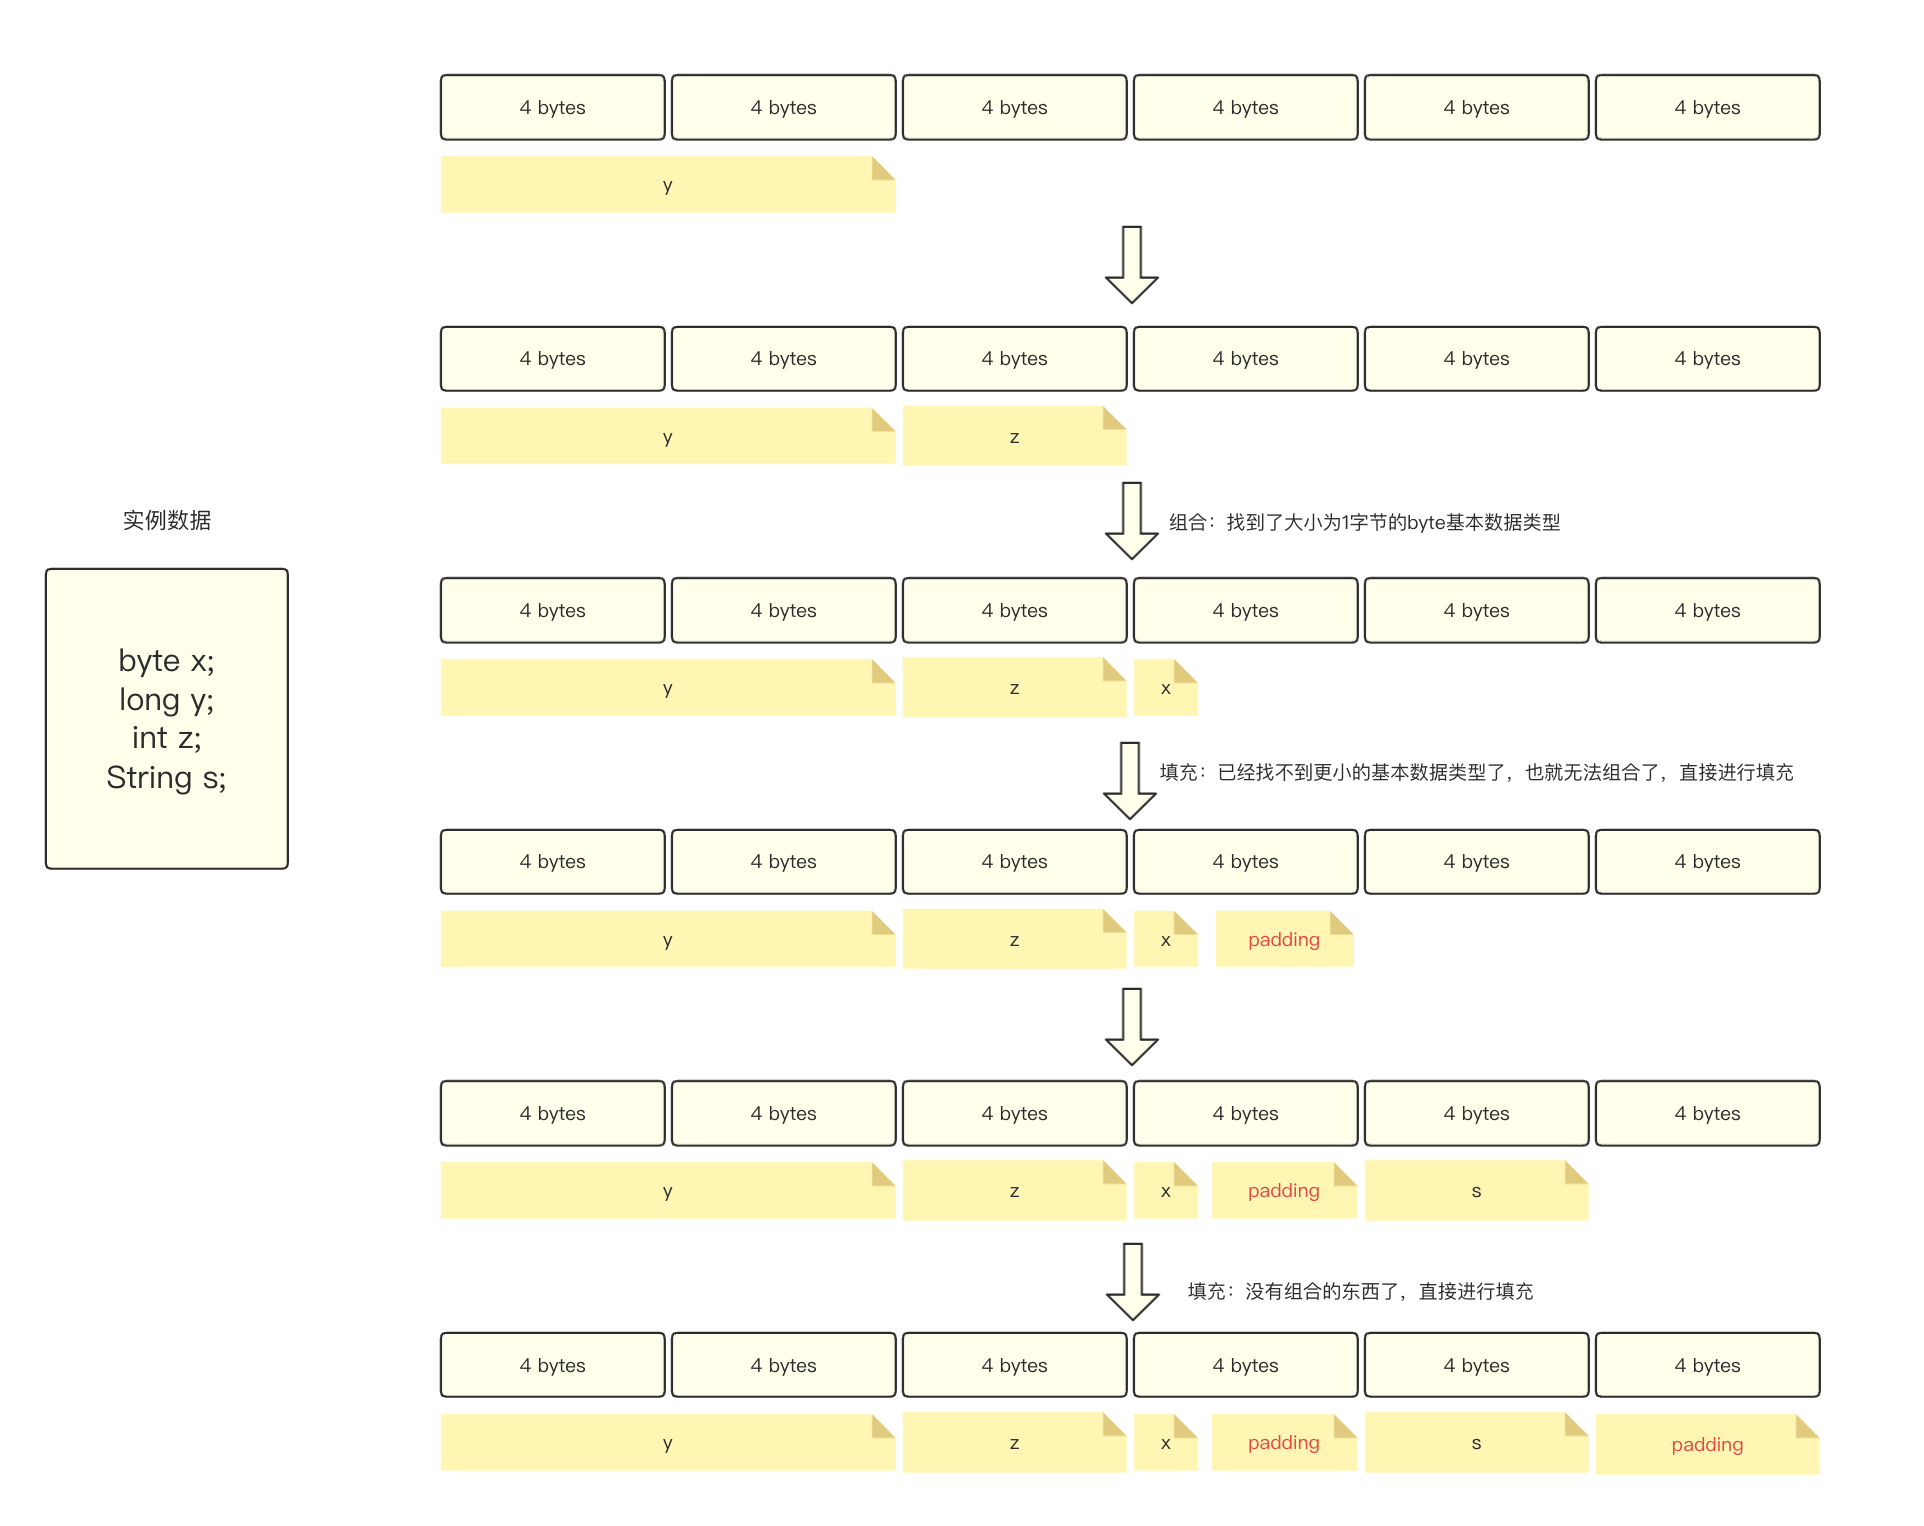
\includegraphics[
%     angle=-45,
%     origin=lb,
%     width=0.9\textwidth]{内存对齐案例}
% \end{center}
\begin{figure}[ht]
    \centering
    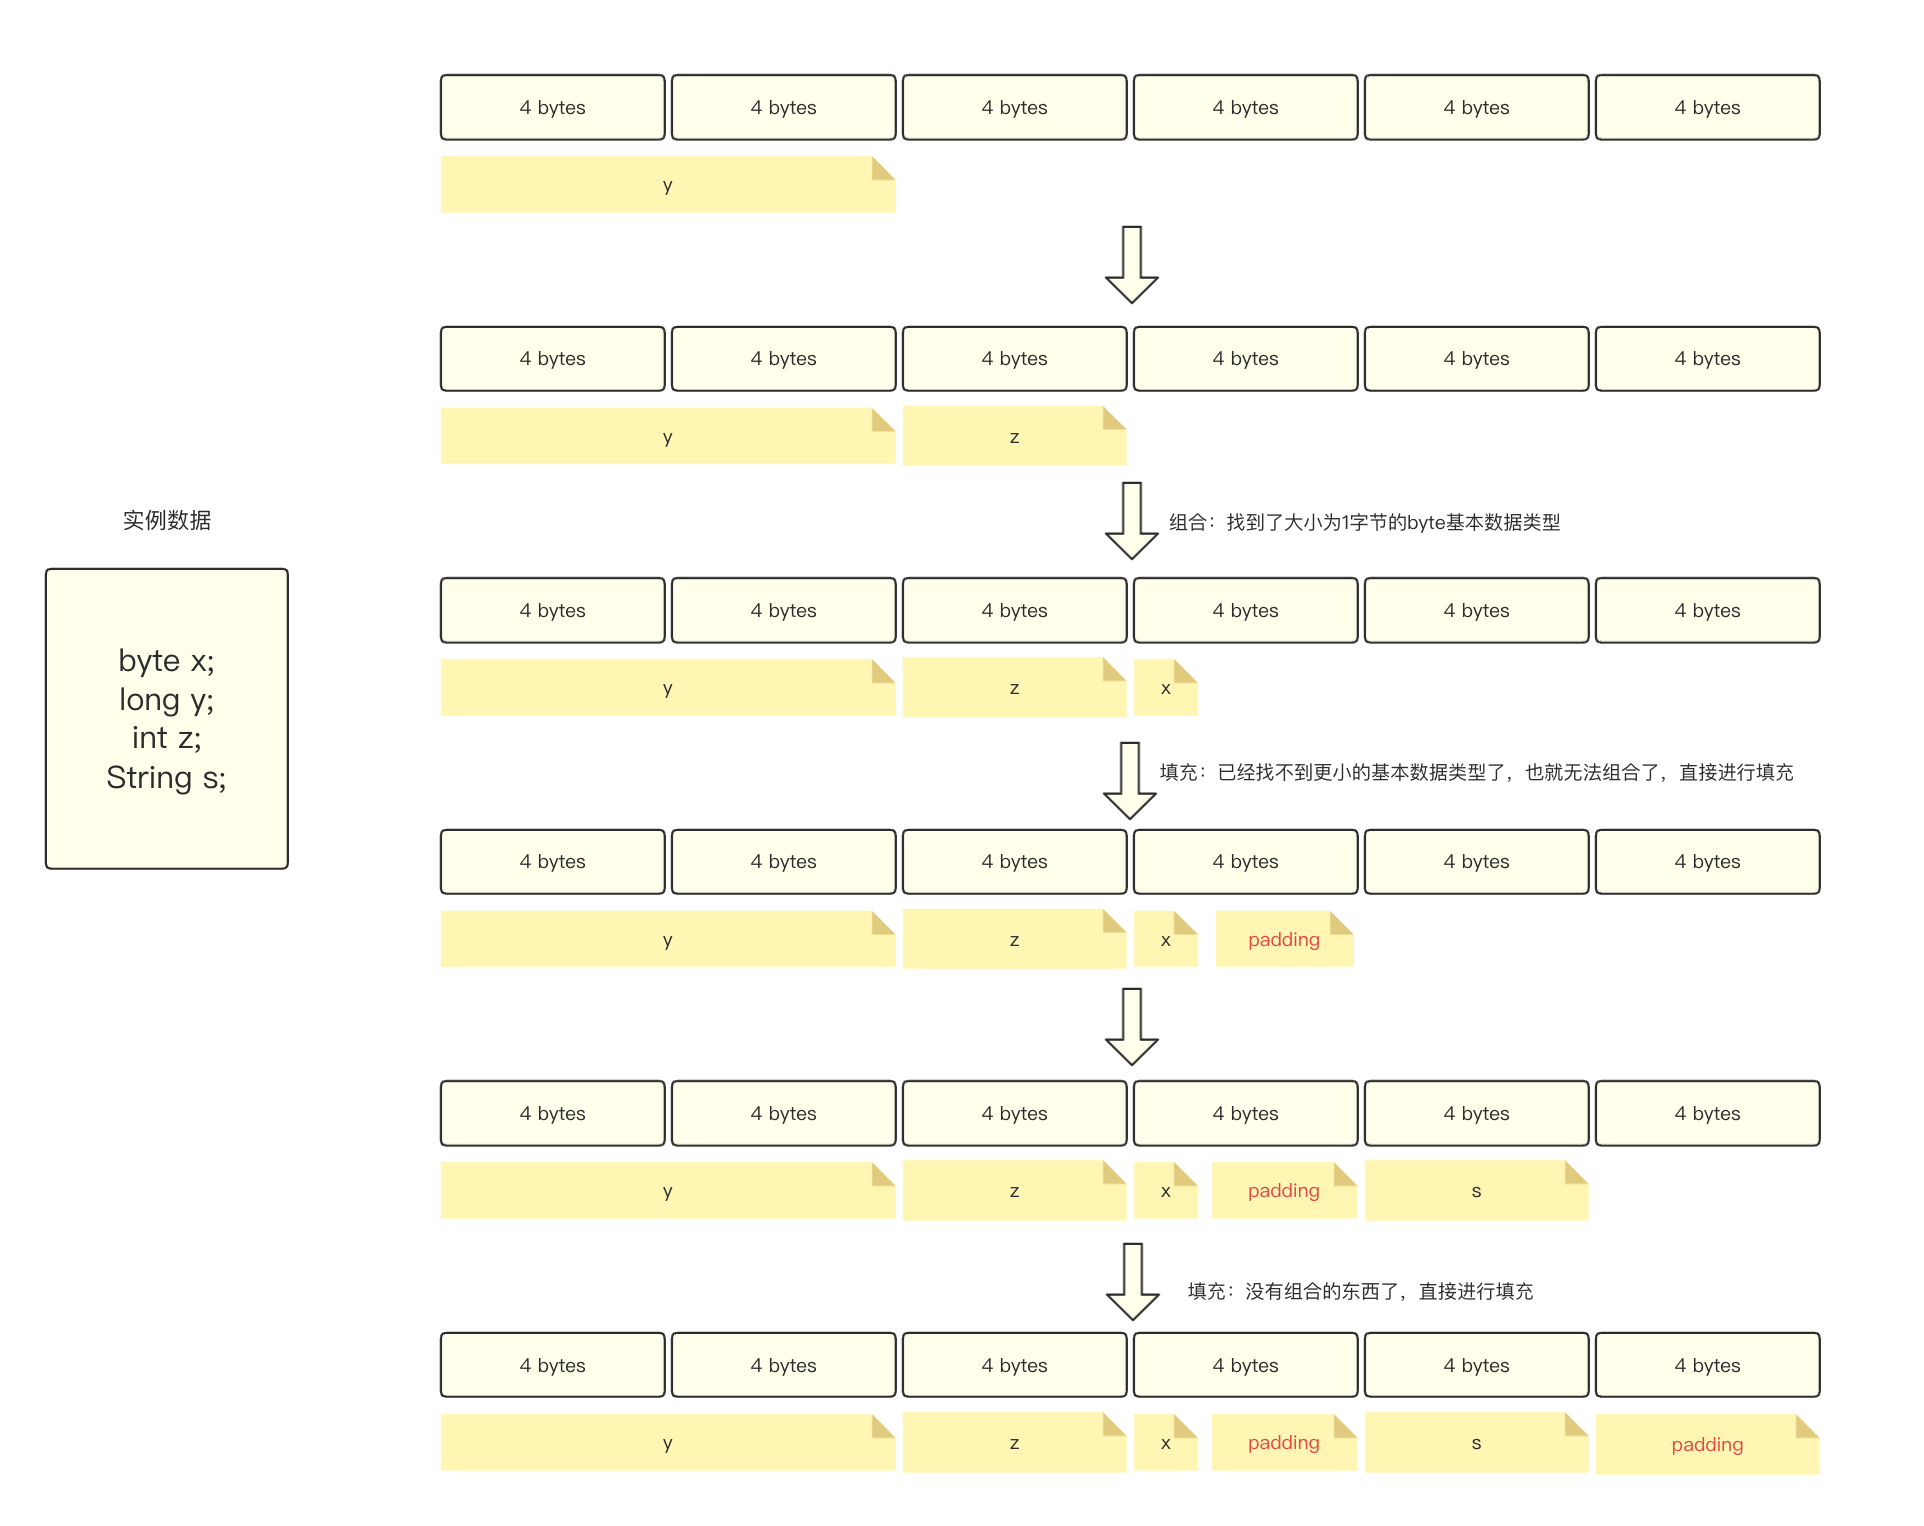
\includegraphics[width=0.9\textwidth]{内存对齐案例}
    \caption{内存对齐案例}
    \label{fig:1}
\end{figure}

这是我们定义的代码\autoref{code:1}:
\begin{lstlisting}[
    language=Java, 
    firstnumber=100, 
    linewidth=1.0\linewidth, 
    caption=code,
    label=code:1,
   ]
    // Java code example
    public class Main {
        public static void main(String[] args) throws Exception {
            // 注释
            StreamingExecutionEnvironment env = 
                    StreamingExecutionEnvironment.getExecutionEnvironment();
            env.execute();
        }
    }
\end{lstlisting}

\end{document}